\section{Introduction}

\subsection{Background}
The Liverpool Telescope (LT) is a fully robotic 2 meter astronomical telescope situated at the Observatorio de los Roches de los Muchacos on La Palma in the Canary Islands. It operates without supervision, controlled by an integrated suite of software systems. The Robotic Control System (RCS) is responsible for deciding on the mode of operation and for protecting the telescope, it controls the telescope and its instruments and receives environmental information via a number of lower level subsystems. The Telescope Control System (TCS) is responsible for slewing the telescope axes onto targets and for tracking them through the night. The Instrument Control Systems (ICS) are responsible for configuration of the suite of scientific instruments, taking exposures, reading out, saving to disk and control of a realtime data reduction pipeline (DPRT). The Scheduler is a component of the Observer Support System (OSS) - DEFINE. 

The RCS makes requests to the scheduler at various times for groups of observations to perform. These are then executed and results reported back to the OSS. Observations specified by astronomers who have been allocated time, are stored in the Phase2 Observing Database (ODB) maintained by the OSS. The observation requests include all the information required to perform the observations - target location, instrument selection and configuration, exposure times etc. In addition a number of constraints are specified - time constraints determine when and how often the observations should be performed, observing constraints specify under what environmental conditions the observations may be performed - e.g. only if the target is above a certain elevation or when the \emph{seeing} is better than a specified level. User-specified QOS metrics define the acceptable levels of observation quality and regularity. 

The telescope operates in an uncertain environment \begin{inparaenum} \item availability is influenced by weather conditions (it does not open when there is rain, high humidity or extreme or gusting wind), \item at times the telescope may be \emph{taken over} by an external agenty \cite{xxx} (TOSA) to investigate \emph{targets-of-opportunity}, \item engineering work must be scheduled in at various times, \item there are the inevitable and unexpected downtime due to software and hardware faults, \item atmospheric conditions which constrain the choice of available observation can change over short timescales, \item observation requests can arrive in the database or be removed or modified at any time \end{inparaenum}. These factors make it difficult to make long term scheduling commitments with any chance of success.

\cite{steele97control} have defined a series of ?characteristics? that can contribute to a \emph{good} schedule. They mention fairness (of time allocations between various committees), efficiency (quality of observations, minimization of idle time) and feasibility (is the target visible).

First version of scheduler \cite{fraser04scheduling} is a simple despatch scheduler which uses an objective function formed using a weighted sum of metrics.
Describe the scheduler as candidate selection then application of metrics (leave gory details till later). A full search of the ODB is performed, enabled candidate groups are extracted and scored using a weighted sum of various metrics.

Does it work and how well, what problems - obviously needs imporvment or wouldnt be writing this..

\begin{itemize}
\item inefficient - need to call scheduler each time a group completes/fails.
\item obscure - dont know why decisions are being made - why g-1 and not g-2 selected.
\item suboptimal - just select best group now - no consideration of what next = local optimization.
\item difficult - how do we select the best relative weighting for metrics?.
\end{itemize}

How can we improve..
look at multiobject optimization \cite{silva04multiobjective} - very interesting. \cite{bresina95expected} deals with look-ahead and how improves qualities or metrics.

Say what these mean i.e for what will be doing - adaptive/learning, accountable (user-prefs), dispatch, predictive, lookahead, max utility,

i.e. blah blah - an adaptive scheduler will ... use of prediction to estimate likelihood of conditions for boosting future reward.. using dispatch because...the MEU theorem and decision thry....


\subsection{Scheduling in context}
Scheduling problem in general defined S+P+E+C - hierarchy, horizons, feedback/cyclic nature of process.

The aim of scheduling is to generate a schedule - this indicates what is to be done, when, and with which resource(s).Scheduling cannot however be considered in isolation, it is part of a hierarchy involving concepts such as planning and execution. In a machine environment there will also be a need to consider aspects of low level control and feedback.  
At some point the distinction between planning, scheduling and execution may become blurred depending on just how we characterize these. In highly dynamic environments planning, scheduling, execution and control may be continuous, interleaved or merged into a single operational \emph{entity} - better word?.

\begin{description}
\item[Scheduling] involves taking decisions regarding the allocation of available capacity or resources (equipment, personnel, space) to jobs, activities, tasks or customers over time. Scheduling thus results in a time-phased plan, or schedule of activities.

\item[Planning] involves the determination of the goals and objectives of an enterprise and the selection, through a systematic consideration of alternatives, of the policies, programs and procedures for achieving them. An activity devoted to clearly identifying, defining, and determining courses of action, before their initiation, necessary to achieve predetermined goals and objectives.

Planning is typically a long term activity - we define the term planning horizon as the period over which a plan is made or is expected to be of some utility in achieving its set out goals/objectives. Planning takes a global view of the enterprise, it may set targets to be achieved by the enterprise e.g. in the form of objective functions or the specification of constraints and preferences to be considered by lower layers. These goals may be somewhat imprecise or abstract - we are not deciding what to do when so much as what sort of things we want to do and how well we want to achieve them. 

We can usefully subdivide planning into several different horizons \cite{xxx} - these are by no means set in stone and more/fewer horizons may be more suited to specific enterprises. The precision of the objectives becomes more focused and the time span decreases as we move down the hierarchy \cite{chien00aspen}??

\begin{description}
\item[Strategic] horizon involves the creation of plans to cover very long periods of time. Typically this could be over a year or more and could at its most extreme represent the entire lifetime of an enterprise. 
\item[Tactical] horizon plans are designed to cover medium periods e.g. a semester on a telescope,  weekly or monthly production targets in factory.
\item[Operational] horizon plans are short term plans designed to allow an enterprise to function function, typically they cover the standard work-period of the enterprise e.g. a night's observing at a telescope, a shift at a factory.
\end{description}

\item[Execution] is the carrying out of the tasks assigned by the scheduler or planner by the enterprise - i.e. its normal operating procesdures. Execution may itself involve decomposition of assigned tasks, recovery from error or reaction to unexpected events.


\end{description}

Formally we shall define the scheduling problem with respect to the following structures:-

\begin{itemize}
\item A database, repository, queue or pool of tasks/jobs/activities $\mathbf{T}$ which are to be performed. This could be a set of observations by a telescope, processes on a computer, components to be manufactured in a factory, surgical operations to be performed in a hospital, blocks of trees to be felled in a forest. The pool of tasks may be static or dynamic, with new tasks inserted and uncompleted tasks removed while the execution is underway.

 \item A set of constraints $\mathbf{C}$ associated with the jobs - these may be \emph{unary} (limits on a single variable or resource e.g. $task_i$ must start between $t_1$ and $t_2$), \emph{binary} (linking the values of 2 variables - e.g. predecence $task_i$ must start before $task_j$ ) or may involve relationships between several problem variables. They may be further divided into:-
y\begin{description} 
\item[hard constraints] which must be guaranteed to be satisfied by a valid schedule, e.g. 
\begin{enumerate}
\item $task_i$ must be completed by latest finish time $lft_i$.
\item only 2 tasks can execute on $machine_y$ simultaneously.
\item there must be a gap of at least $t_{ij}$ between execution of $task_i$ and $task_j$.
\item $team_k$ cannot work more than $max_k$ hours in any day.
\end{enumerate}

\cite{sadeh91lookahead} and \cite{fox83thesis} define the following classes of constraints:-
\begin{itemize}
 \item  precedence constraints - describe
 \item  resource usage constraints - describe
 \item  many others - (see Fox paper).
\end{itemize}

 \item[soft constraints] or preferences which should be satisfied as far as possible but which are capable of relaxation to permit a feasible schedule to be derived. When relaxing constraints it is usual to associate a cost to the degree of relaxation, this  may be folded into the global objective function. The manner in which such relaxation occurs is likely to influence the search heuristics.
 (a list of examples here)
\begin{itemize}
 \item A telescope suffers from changes to \emph{seeing} due to turbulent motion of the atmosphere- some observations may have constraints which state they cannot be executed if the seeing is worse than $x$. 
 \item A machine in a factory may have a capacity which is determined by the current power levels or time of day.
 \item and another.
\end{itemize}

\end{description}

\item A set of resources $\mathbf{R}$ to assign to the tasks. e.g. a telescope or one of several observatories for performing the observations, a production line or machine to make the components, a team of lumberjacks to fell the blocks of tree, a surgical team to perform the operations.

\item A set of goals $\mathbf{G}$ which we are trying to achieve by performing these tasks. Goals may be specified in terms such as the standard measures from the CSP literature:- \emph{min-slack}, \emph{max-throughput}, \emph{min-tardiness}, or may be set out as objective functions to be maximized. Either way we need to be able to extract appropriate quality parameters from the schedule. 

\item The environment $\mathbf{E}$ in which the scheduler lives and which can influence the execution of the tasks and can change the goals. (list of examples plus refs- ) 

Environmental variables may be:- 

\begin{itemize}
  \item static - constant in time (telescope's elevation limit, number of processors).
  \item dynamic - changing in time (telescope's current azimuth, current instrument selection, etc).

These may further be classified as:-
\begin{itemize}
  \item deterministic - always known or predictable (e.g. position of the moon which affects sky-brightness and integration times, is always calculable).
  \item stochastic - randomly variable - (examples).
  \item chaotic - e.g. weather \cite{lorenz63npflow}, atmospheric seeing \cite{jorgenson91attractor}.
\end{itemize}
\end{itemize}

\end{itemize}

Scheduling may be divided into 2 sub-problems - the satisfycing problem consists of finding a schedule which satisfies the hard constraints i.e. all the tasks are assigned to a valid time slot without regard to preferences - we refer to this as a feasible schedule. Such a schedule may contain significant amounts of slack time (when no tasks are being performed) or under-utilization of resources - such schedules are generally inefficient but that may be all that is required - these problems may be represented as constraint satisfaction problems (CSP). The optimization problem consists of finding a schedule which is both feasible and achieves its goals as layed down by the soft-constraints whilst maximizing an objective function (or minimizing a cost function which is equivelent). We will refer to this as an optimal schedule and may be represented as a constraint optimization problem (COP). 

\subsection{Classification of scheduling problems}
Some ideas on classification of scheduling problems:-

\begin{description}
\item[Integration Depth] How much of the hierarchy of planning, scheduling, execution (and control) is involved and is there feedback and from/to which level(s).
\item[Flexibility] Are the results of the scheduling (i.e. the generated schedule to be followed) fixed or does it contain some flexibility. This may be in the form of temporal or resource assignment flexibility (windows in a fixed execution path) or a graph of multiple execution futures - i.e. contingency/redundancy .
\item[Proactive/reactive] Is the scheduling performed online or offline. ()Better name? - proactive at one end, reactive at other end of a scale)
\item[Method] Constructive or repair based, DDS is \emph{sort of} in between. Distributed techniques may confound this?. 
\item[Horizon] The time period or number of tasks over which the schedule is expected to be followed.
\item[Completeness] The number of tasks from the set of available/assignable tasks to insert into the schedule.
We can extract the following progression:-
\begin{enumerate}
\item Despatcher - Scheduler seeks the \emph{best} single task to perform from the set of assignable tasks at an instant.
\item Short Horizon - Scheduler selects a sequence of tasks from a subset of the assignable set to perform.
\item Complete - Scheduler must assign all assignable tasks.
\end{enumerate}
\end{description}

Note: In this scheme DDS is \emph{variable depth (typically S with feedback from E), neccessarily fixed, online with horizon $=$ 1 task, using a repair? based method}. 

Q:- What advantages/disadvantages do these measures convey - integrate into paras above?

Notes:- Completness/horizon - how do we determine the length of the horizon or do we select a subset of tasks from pool to execute over a horizon? Several ways:-
\begin{itemize}
\item Use knowledge of the environment dynamics and uncertainty in execution times to choose a \emph{hard-coded} horizon length.
\item Adaptively select horizon length from measured environment dynamics.
\item Use higher level goal-based planner to select a subset of pool for execution over the next horizon.
\item Combine the last 2.
\end{itemize}


\subsection{Constraint Satisfaction Techniques}

A constraint satisfaction problem (CSP) comprises:- A set $\mathbf{X} = \{x_i\}$ of variables over a set of domains $\mathbf{D} = \{d_i\}$ these may be continuous or discrete and bounded or unbounded and a set $\mathbf{C} = \{c_i\}$ of constraints on and between the variables that restrict the possible value assignments. A solution comprises an assignment of values from $\mathbf{D}$ to all the variables in $\mathbf{X}$ subject to $\mathbf{C}$. Further in an optimization problem the solution should maximize an objective function $F(\mathbf{X})$. A CSP may be represented as a directed graph in which the arcs represent constraint relationships between the variables represented as nodes. To represent a scheduling problem as a CSP the variables are identified as the tasks to be assigned time-slots from domains of available times. The objective function is a measure of the quality of the schedule.

   \begin{figure}[h]
   \begin{center}
   \includegraphics[height=6cm]{figures/placeholder.eps}
   \end{center}
   \label{fig:object} 
   \caption[Scheduling as a CSP.] 
   {Scheduling problem represented as a CSP graph with time-slot assignments (domains) for tasks (vars).}
   \end{figure} 


Solving scheduling as a CSP - 2 techniques have evolved - constructive techniques based on backtracking search from starting from an empty schedule, build up partial schedule by selecting a task and assigning a value from its available domain, check for consistency then onto next task. Keep going till hit deadend - no assignment of variable will allow progress. Then backtrack to last decision (assignment) and change. Uninformed backtracking typically requires $O(n!)$. In contrast, the repair technique starts with a fully built but typically inconsistent and suboptimal schedule. The technique then involves an iterative cycle of task retraction and re-assignment until all tasks are assigned and all constraints are satisfied. If optimization is required the objective function is measured at each cycle to check for improvment. The objective may also guide the search heuristics.



\subsection{Problem definition}
Detailed specification of observing requirements and what trying to do and what sent to RCS and what comes back- - RCS does task decomposition, it is the executor. include linked groups, sequencing 

Specific nomenclature/terminology and symbols that will be used hereafter.



The Phase 2 Observing Database (ODB) (see Fig.~\ref{fig:phase2-architecture}) contains details of all the programs of observations. These details are supplied by astronomers using external tools \cite{clayandfraser06tbd} or are generated by external intelligent agents \cite{xxx} (TEA).

   \begin{figure}[h]
   \begin{center}
   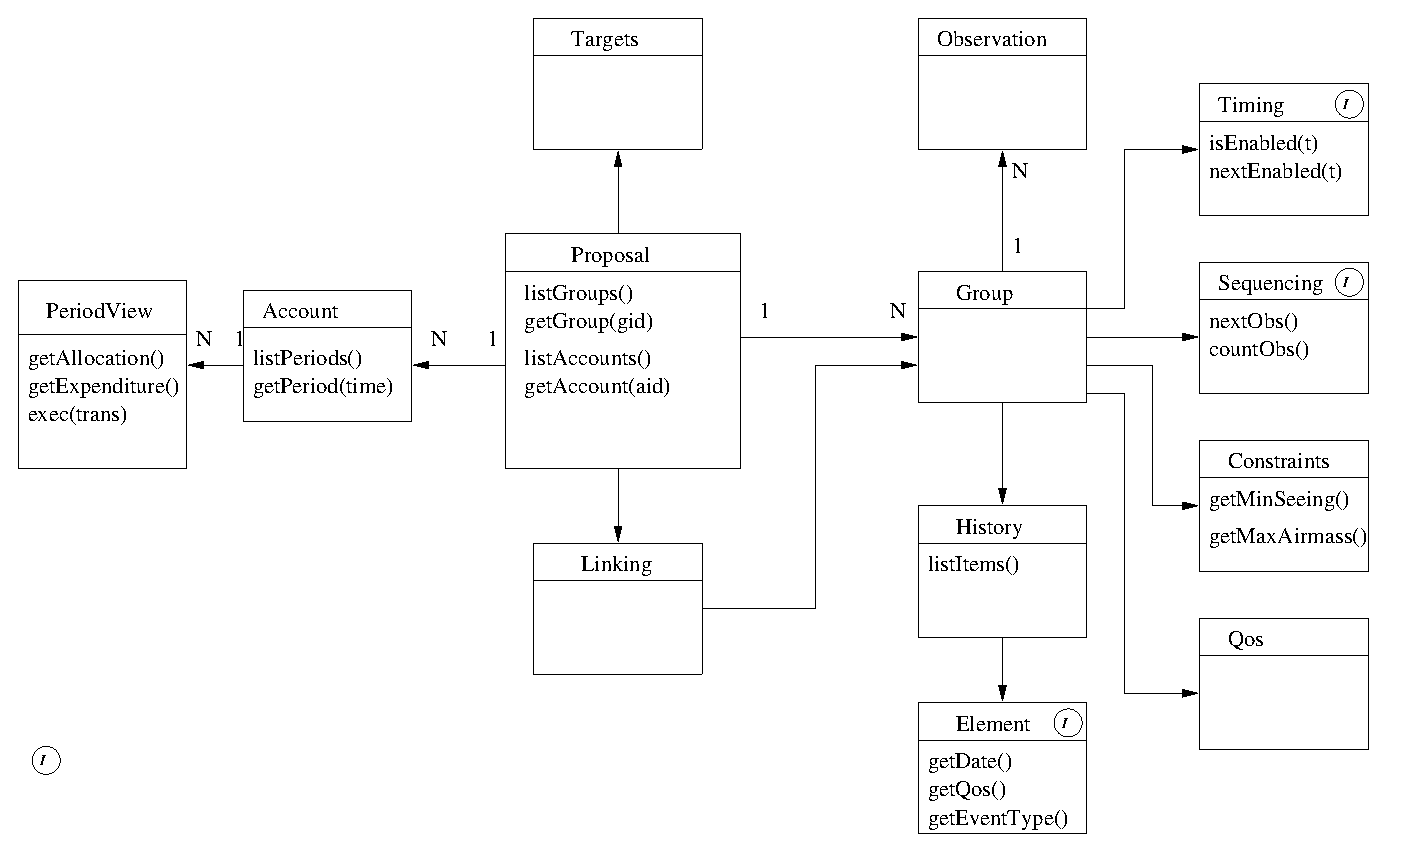
\includegraphics[height=6cm]{figures/phase2_architecture.eps}
   \end{center}
  
   \caption[Phase2 Architecture.] 
   {The Phase2 Observing Database (ODB) contains details of {\tt Proposals}, {\tt Groups} of {\tt Observations}, {\tt Accounting}, {\tt Linking}, {\tt Targets} and {\tt ExecutionHistory}..blah..blah.}
   \label{fig:phase2-architecture} 
   \end{figure} 

Proposals represent an astronomers observing program and correspond directly with the ?general definition? of a TAG allocated proposal. A proposal collects information required to perform the client's observations and time and resource accounting.  Programs collect together a number of different proposals for sharing of resource allocation. A proposal may participate in several programs. The unit of scheduling is termed a group and consists of the specifications of the observations, timing requirements, sequencing, observing condition constraints and quality of service metrics. Groups within a proposal may be linked in various ways (Fig.~\ref{fig:group-linking} contains details of some of these relationships.


   \begin{figure}[h]
   \begin{center}
   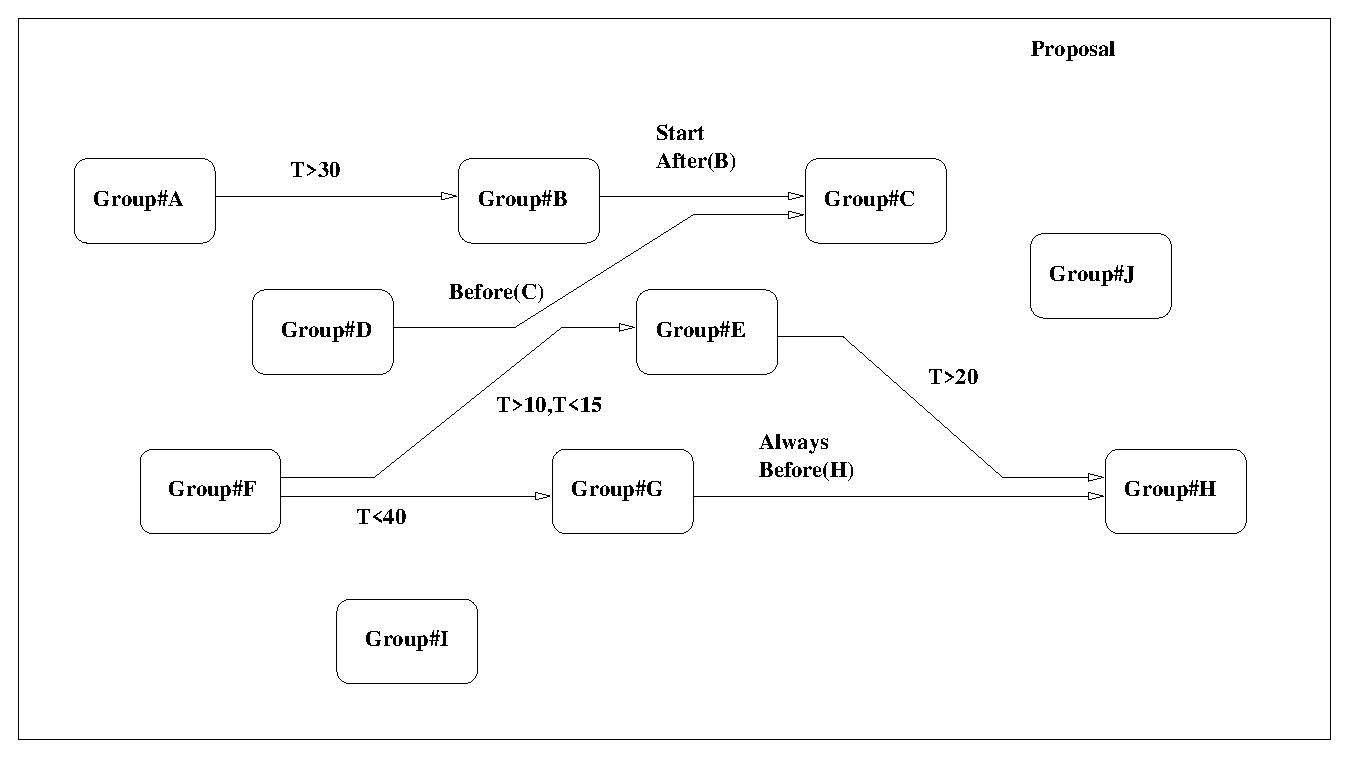
\includegraphics[height=6cm]{figures/group_linking.eps}
   \end{center}
  
   \caption[Group Linking.] 
   {Groups within a proposal may be linked in various ways. The constraint between {\bf Group\#A} and {\bf Group\#B} states that a {\bf Group\#B} cannot be executed unless a {\bf Group\#A} was executed at least 30 units earlier. The constraint between Groups {\bf \#C} and {\bf \#D} states that C should only be executed if D is able to be executed between 20 and 40 units later and requires the ability of the scheduler to predict future group enablement.}
   \label{fig:group-linking} 
   \end{figure} 


Each group has a set of enablement windows $E={e_i}$ which represent the intervals during which it should be observed if possible - these are obtained from the group's \texttt{TimeConstraints}, e.g. make this observation sometime between t1 and t2. As an added complication these may be cyclic - e.g. perform this observation once every 3 hours between t1 and t2. Some observations have fixed time constraints (do this at t3) or sliding fixed time constraints (do this at t1 or t2 or t3). 

The times when the group can actually be observed are further constrained by a number of factors:-
\begin{itemize}
\item Observations are only performed at night - in some cases we further restrict this to the period between evening and morning astronomical twilight.

\item Environmental constraints, some are deterministic e.g. only observe this target if the moon is greater than distance \emph{x} away from the target or only observe if the target is above elevation \emph{y}. Others are less predictable, e.g. only observe this target if the atmospheric seeing is less than \emph{z} arc seconds. 

\item Observations cannot be made during bad weather (the dome is closed to protect the instruments) and there is no point observing in cloudy conditions

\item There are unpredictable target-of-opportunity interrupts where external intelligent agents may take over the telescope for a period with no advance warning

\item There are certain periods, usually known in advance when the telescope is unavailable due to engineering or local or remote manual observing.

\end{itemize}

Taken together these result in considerable uncertainty in the time spans available for observing (active windows). In such a dynamic environment any advanced planning can become rapidly out of date. 


The figures below illustrate 2 scenarios which might arise. 1- period monitor, 2- long flexible - one with real weather superimposed would be spiffing - this is tricky!

%
INSERT FIGURE showing enablement intervals and stuff..
%

A schedule can be any of the following in increasing degree of generalization:-
\begin{itemize}
\item A single group to execute.
\item A series of groups with valid time windows.
\item A tree of alternative groups with time windows and validity conditions.
\end{itemize}

Note: These paras need hacking about..

We choose to describe a schedule using a graph where each node \emph{i} represents a tuple of the form $<g_i,T_i,C_i,S>$, where $g_i$ is a group, $T_i$ is a time interval $[est_i, lft_i]$ spanning the earliest start time and latest finish time for $g_i$, $C_i$ represents a set of boolean constraints $\{c_{ij}\}$ on the current (at the time of execution) environmental conditions under which which the group may execute and $S$ is a priority score which allows a decision to be made when several groups can be executed at a given decision point. An example of a set $C$ might be $C_k = \{seeing < 0.8, skybright < 0.5\}$ indicating that group $g_k$ may be performed if the current atmospheric conditions satisfy the 2 constraints specified. The schedule must be executed in sequence by following a path through the graph from the start node. The duration of each group cannot be determined precisely in advance (though it can be estimated with reasonable accuracy) due to variable acquisition times, slewing and settling of directional and rotator axes and instrument internal configuration - we shall attempt to characterize this as part of the project.

The depth (path length) of the schedule we shall define as the \emph{horizon length} and denote $H_L$ - this is the number of groups which can potentially be executed before the scheduler must be invoked again as part of the SEU cycle. In addition we define the \emph{horizon time} $H_T$ as the difference between the largest $lft_k$ in any leaf node of the graph and $est_1$ of the first node and is the longest span we expect the schedule to be valid for. 


As $H_L$ increases, the chances of a schedule breaking (next para) will increase - the characterisation of this parameter under various regimes will constitute part of this project

As a special case \emph{dynamic despatch scheduling} has $H_L=1$ and $C=\emptyset$ indicating that the schedule contains a single group which is by definition executable under the current conditions.

The overall architecture of the system is described in Fig.~\ref{fig:overview_architecture}. The OSS consists of the Scheduler, an UpdateEngine with associated QOS metric thingies and the ODB - the later consisting of Phase2, accounting and execution history databases. The RCS makes information about current conditions and time constraints available to the OSS continuously from which the OSS is able to make predictions about future conditions. When the RCS considers the telescope is available and the conditions suitable for observing it sends a \texttt{request\_schedule} to the OSS. The scheduler interrogates the ODB and selects a schedule suitable for the current and predicted conditions and constraints. The RCS works its way through the schedule by selecting and executing groups. At each decision point a group is selected by comparing the validity time window, constraints and priority score then decomposing the group into a hierarchy of parallel tasks \cite{fraser02robotic} and sending commands to the TCS to control the telescope and to the ICS to configure and control the instrument(s). If a decision point is reached where no group in the schedule can be executed the schedule breaks and the scheduler must be invoked to generate a new schedule. As each group is completed (or fails) \texttt{execution\_results} are sent to the OSS containing information about the execution of the group. The UpdateEngine uses this and the group-specific QOS metrics to update the Accounting and History databases. 

   \begin{figure}[h]
   \begin{center}
   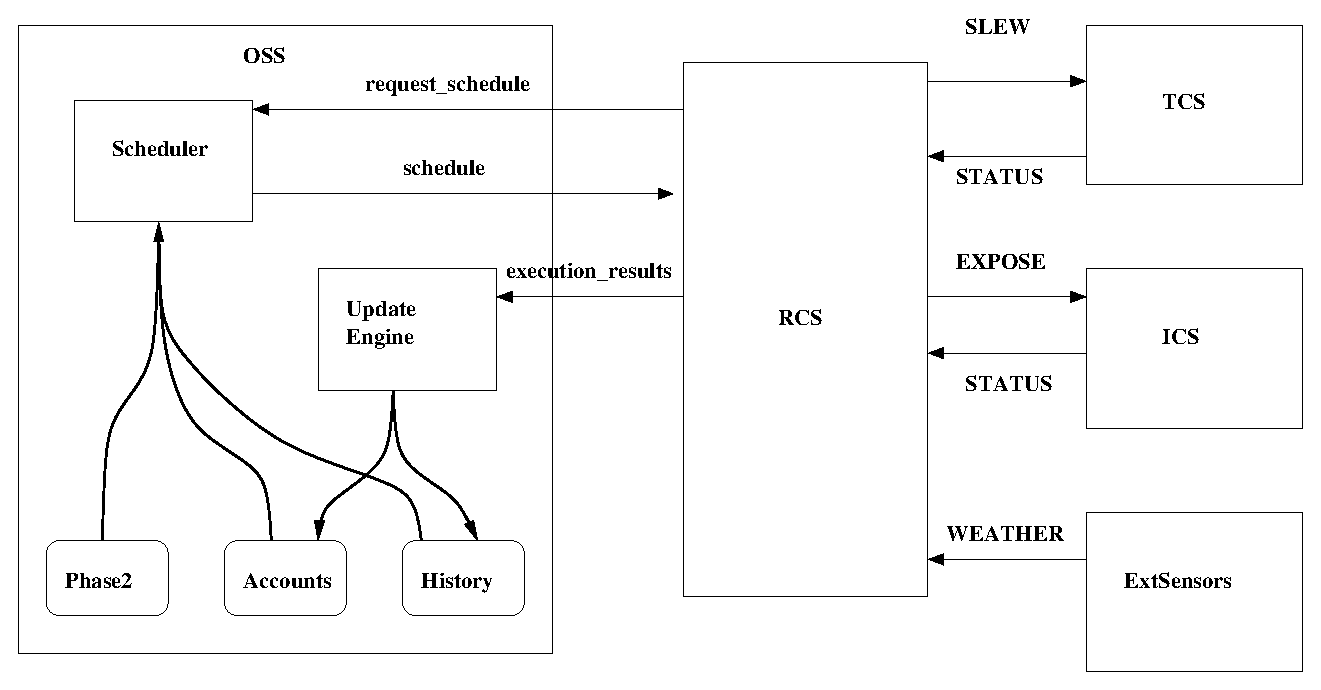
\includegraphics[height=6cm]{figures/overview_architecture.eps}
   \end{center}
  
   \caption[Overview of Architecture.] 
   {Scheduling Engine (SE) uses the Phase2, Accounting and History databases to decide on groups to schedule. On execution of a group the RCS sends results back which are processed by Updating Engine (UE) to update accounting information and QOS Thingy (QT) using group-specific QOS metrics to update history.}
   \label{fig:overview_architecture} 
   \end{figure} 

In the current system the overheads associated with the schedule-execute-update cycle amount to the sum of the schedule generation and instrumentation setup times $t_{sched}$ and $t_{setup}$. This occurs for each cycle i.e. for each group executed. If the group execution time $t_{group} \gg t_{sched}+t_{setup}$ then this is not a great problem. However in the case of groups with short execution times considerable efficiency increases could be achieved by generating a longer schedule sequence with groups chosen so that the setup time between groups is minimized. Real world examples of this scenario have been observed where a pair of short period (in the order of 5 minute) monitoring groups with close targets and with durations of about 2 minutes incurred the full schedule and setup overheads when a pre-defined sequence could have selected the groups to execute in an interleaved fashion with minimal overheads. Another more extreme situation was observed where a single short period monitor was picked to run several times in succession but with the full slew and aquire setup overhead when a pre-defined sequence would have avoided the need to re-aquire the target thus reducing the overhead to almost zero.

\subsection{Research goals}
Quite vague and general - leave details until start of Plan/methodology section after review and before results.

Set the scene and problem statement. Introduce structure of thesis, state contributions 

Reduction of overheads. Flexible schedules. Qos measures. User prefs/metrics, Increase schedule and observation quality. 

